\documentclass{ctexbeamer}

\hypersetup{
  pdfcreator=TeX,
  pdfpagemode=FullScreen,
}

\mode<presentation>{
  \usetheme{Madrid}
}

\title{数据库大作业展示}
\subtitle{百货商店-图书管理系统}
\author{计试2201 梁佳伟\\计试2201 郑诗棪}
\institute[Xi'an Jiaotong University]{
  西安交通大学
}
\date{}

\subject{数据库课程展示}

%整体思想是, 百货商店系统作为一个后台管理, 图书管理系统作为一个给用户呈现的前台


% \AtBeginSubsection[]{
%   \begin{frame}<beamer>{目录}
%     \tableofcontents[currentsection]
%   \end{frame}
% }

\begin{document}

\begin{frame}
  \titlepage
\end{frame}

\section{设计思想}

\subsection{整体设计思想}
\begin{frame}{整体设计思想}
  % 首先我们实现了一个百货商店的框架, 作为商店内部管理的数据系统
  % 在这个框架下, 我们丰富了其中图书部分的信息, 为图书部分提供了用户交互的数据系统

  %
  %
  %

\end{frame}

%%%%%%%%%%%%%%%%%%%%%%%%%%%%%%%%%%%%%%%%%%%%%%%%%%%%%%%%%%%%

\subsection{百货商店概览}
\begin{frame}{百货商店概览}
  % 这部分罗列出百货商店中有哪些功能
  % 使用文字加ER图

  %
  %你写一下
  %

\end{frame}

%%%%%%%%%%%%%%%%%%%%%%%%%%%%%%%%%%%%%%%%%%%%%%%%%%%%%%%%%%%%

\subsection{图书管理系统}
\begin{frame}{图书管理系统}
  %这部分罗列出图书管理系统的功能
  %使用文字加ER图
  %爬虫爬取了3万余本图书信息, 并将其存储在数据库中
  %图书信息如下
  %json文件图
  %ER图
\end{frame}

\section{前端展示}


%%%%%%%%%%%%%%%%%%%%%%%%%%%%%%%%%%%%%%%%%%%%%%%%%%%%%%%%%%

\subsection{百货商店入口}
\begin{frame}{百货商店入口}
  %这部分贴图片



\end{frame}

\subsection{百货商店部分功能}
\begin{frame}{百货商店部分功能}
  %这部分贴图片


\end{frame}



%%%%%%%%%%%%%%%%%%%%%%%%%%%%%%%%%%%%%%%%%%%%%%%%%%%%%%%%%%%


%省略若干部分

% \subsection{图书管理系统功能}
% \begin{frame}{图书管理系统功能}
%   \begin{figure}
%     \centering
%     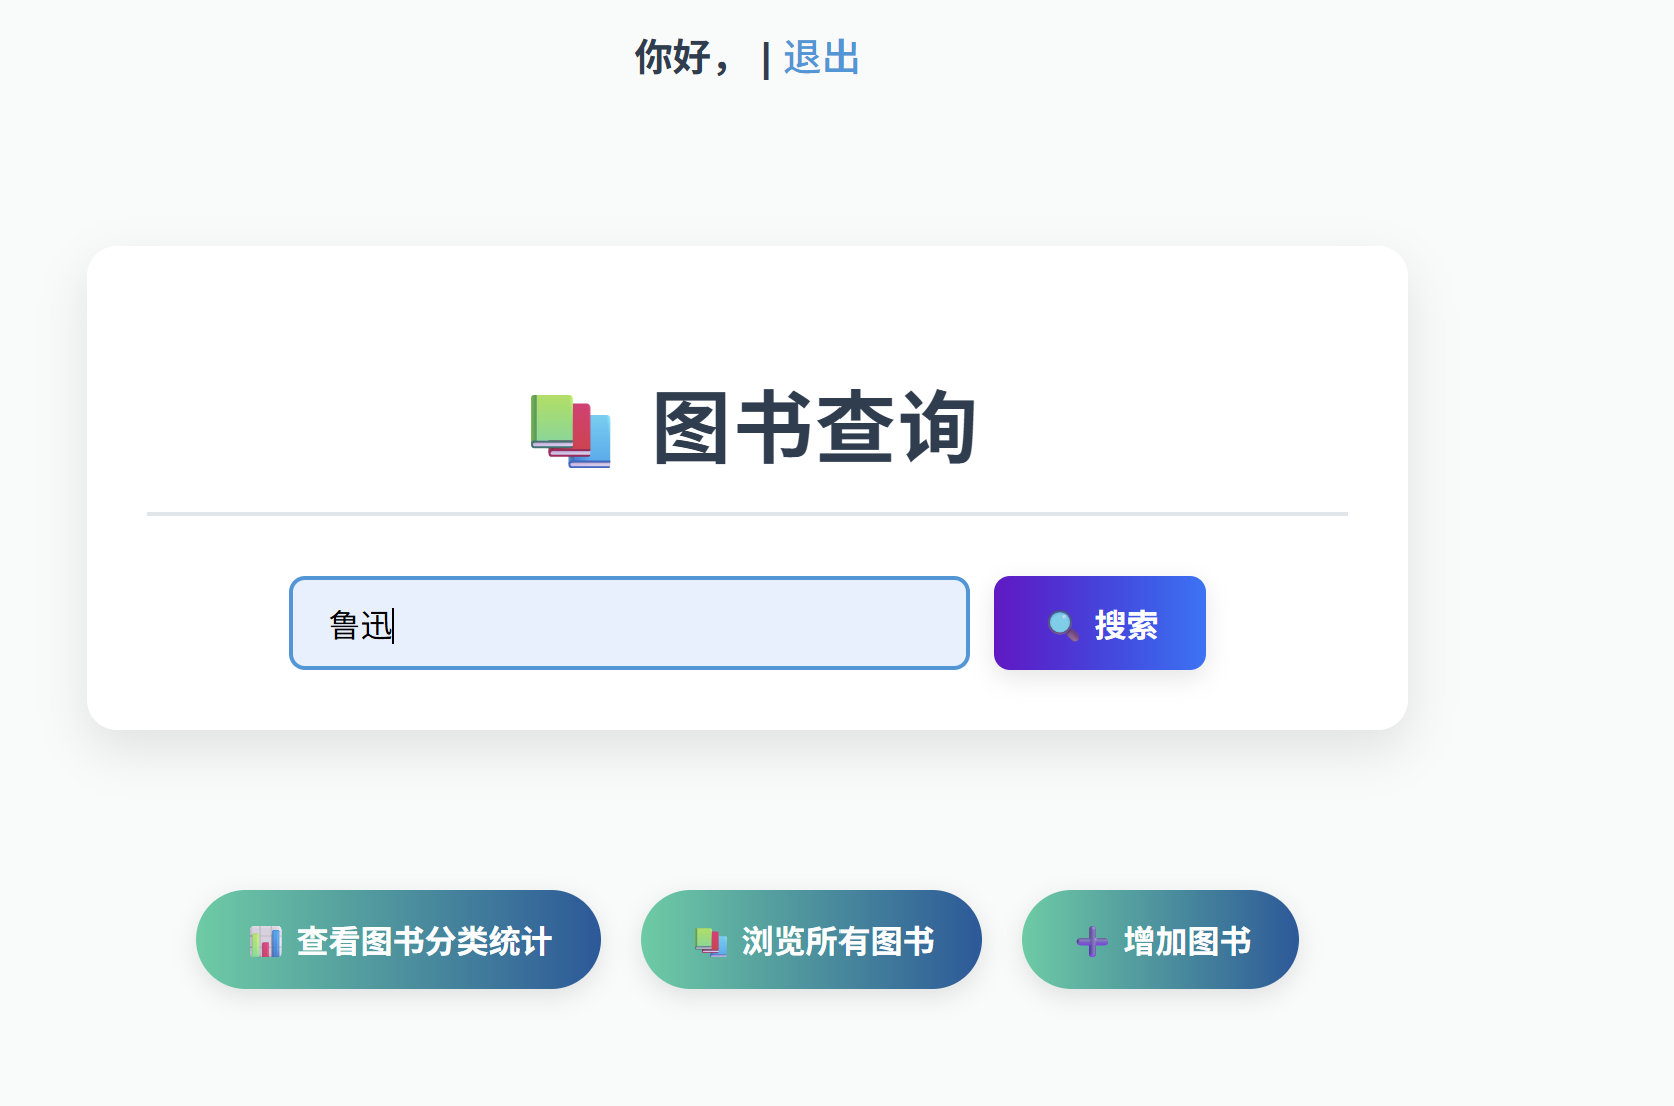
\includegraphics[width=0.8\textwidth]{fig/book1.png}
%   \end{figure}
% \end{frame}

\subsection{图书管理系统部分功能}
\begin{frame}{图书管理系统部分功能}
  \centering
  \begin{minipage}{0.30\textwidth}
    \centering
    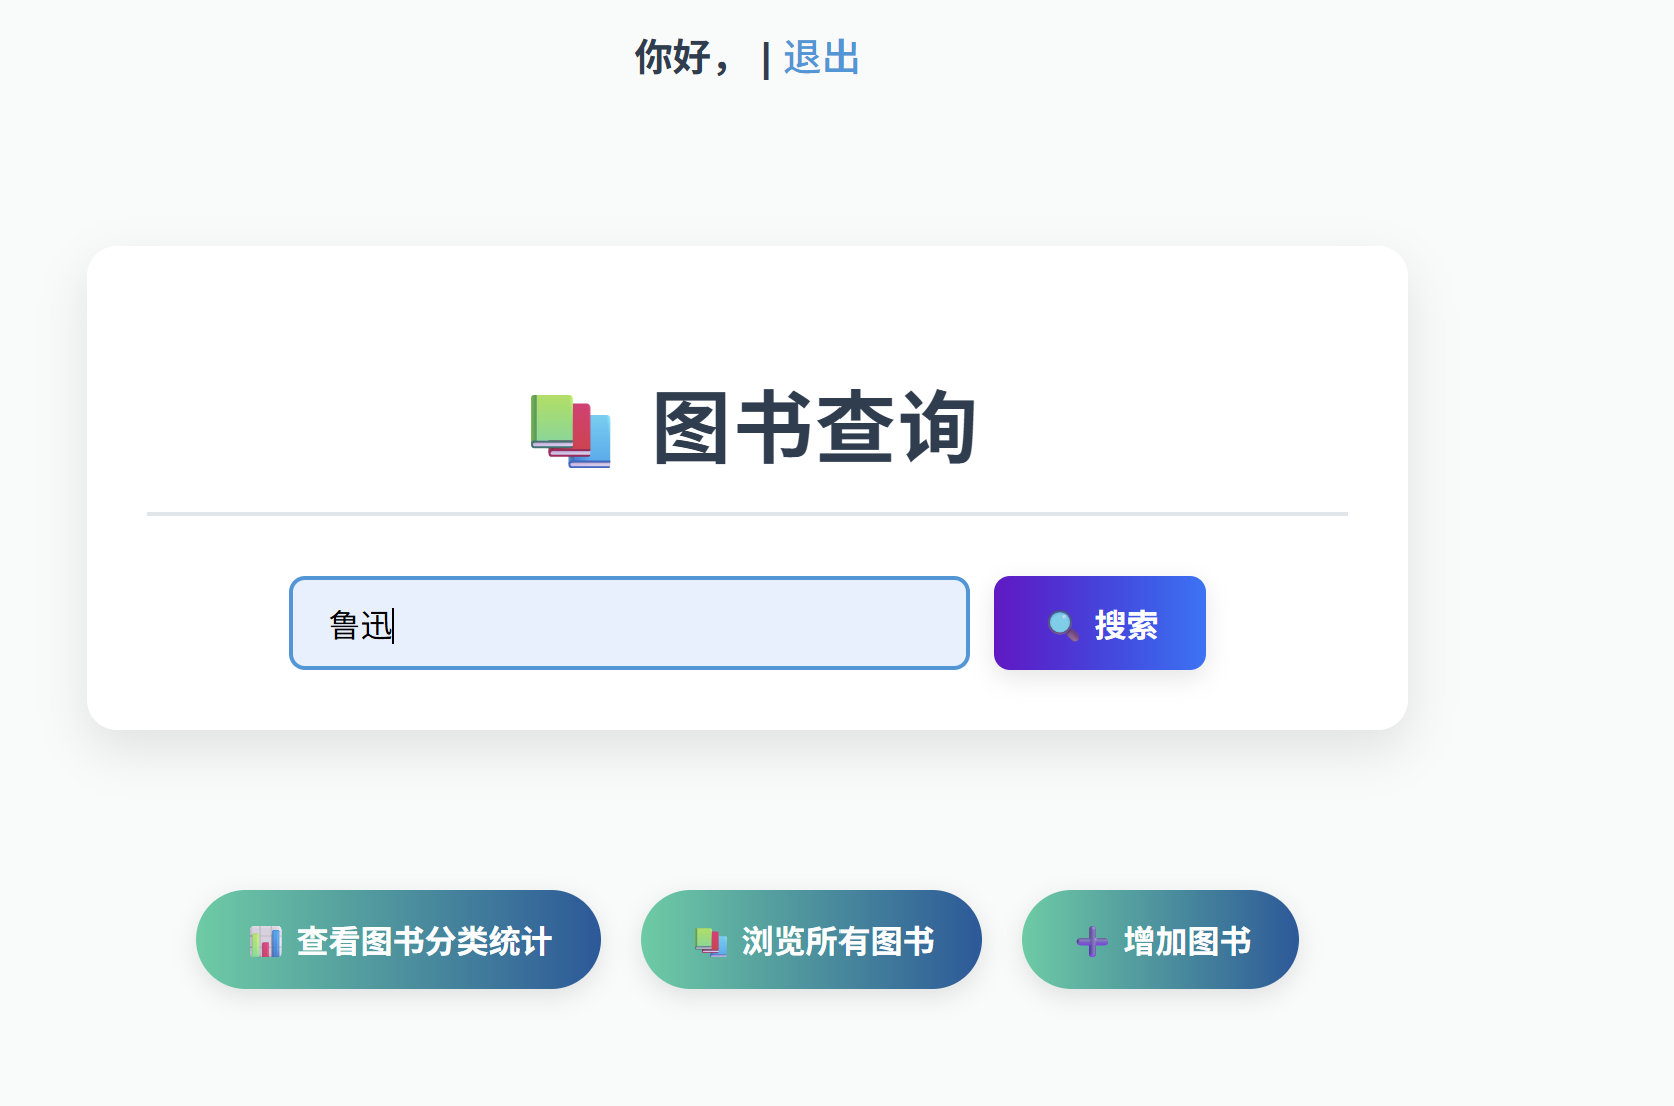
\includegraphics[width=\textwidth]{fig/book1.png} \\
    交互界面
  \end{minipage}
  % \hfill
  \begin{minipage}{0.30\textwidth}
    \centering
    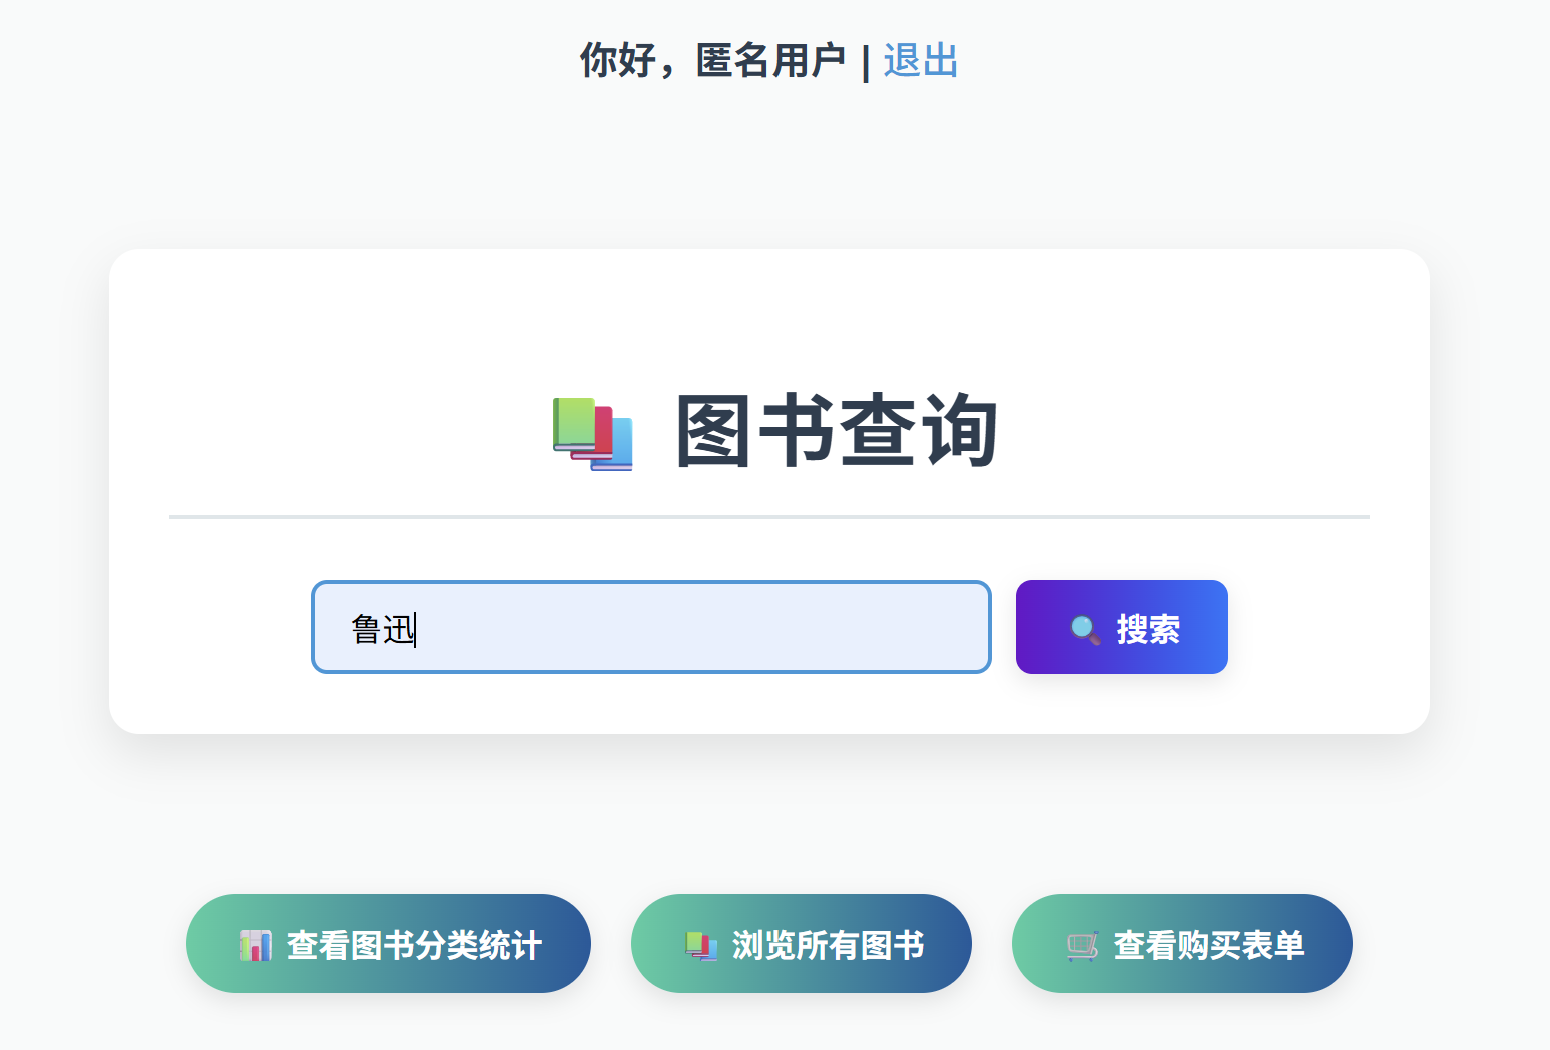
\includegraphics[width=\textwidth]{fig/book2.png} \\
    搜索图书
  \end{minipage}

  \vspace{0.5cm}

  \begin{minipage}{0.30\textwidth}
    \centering
    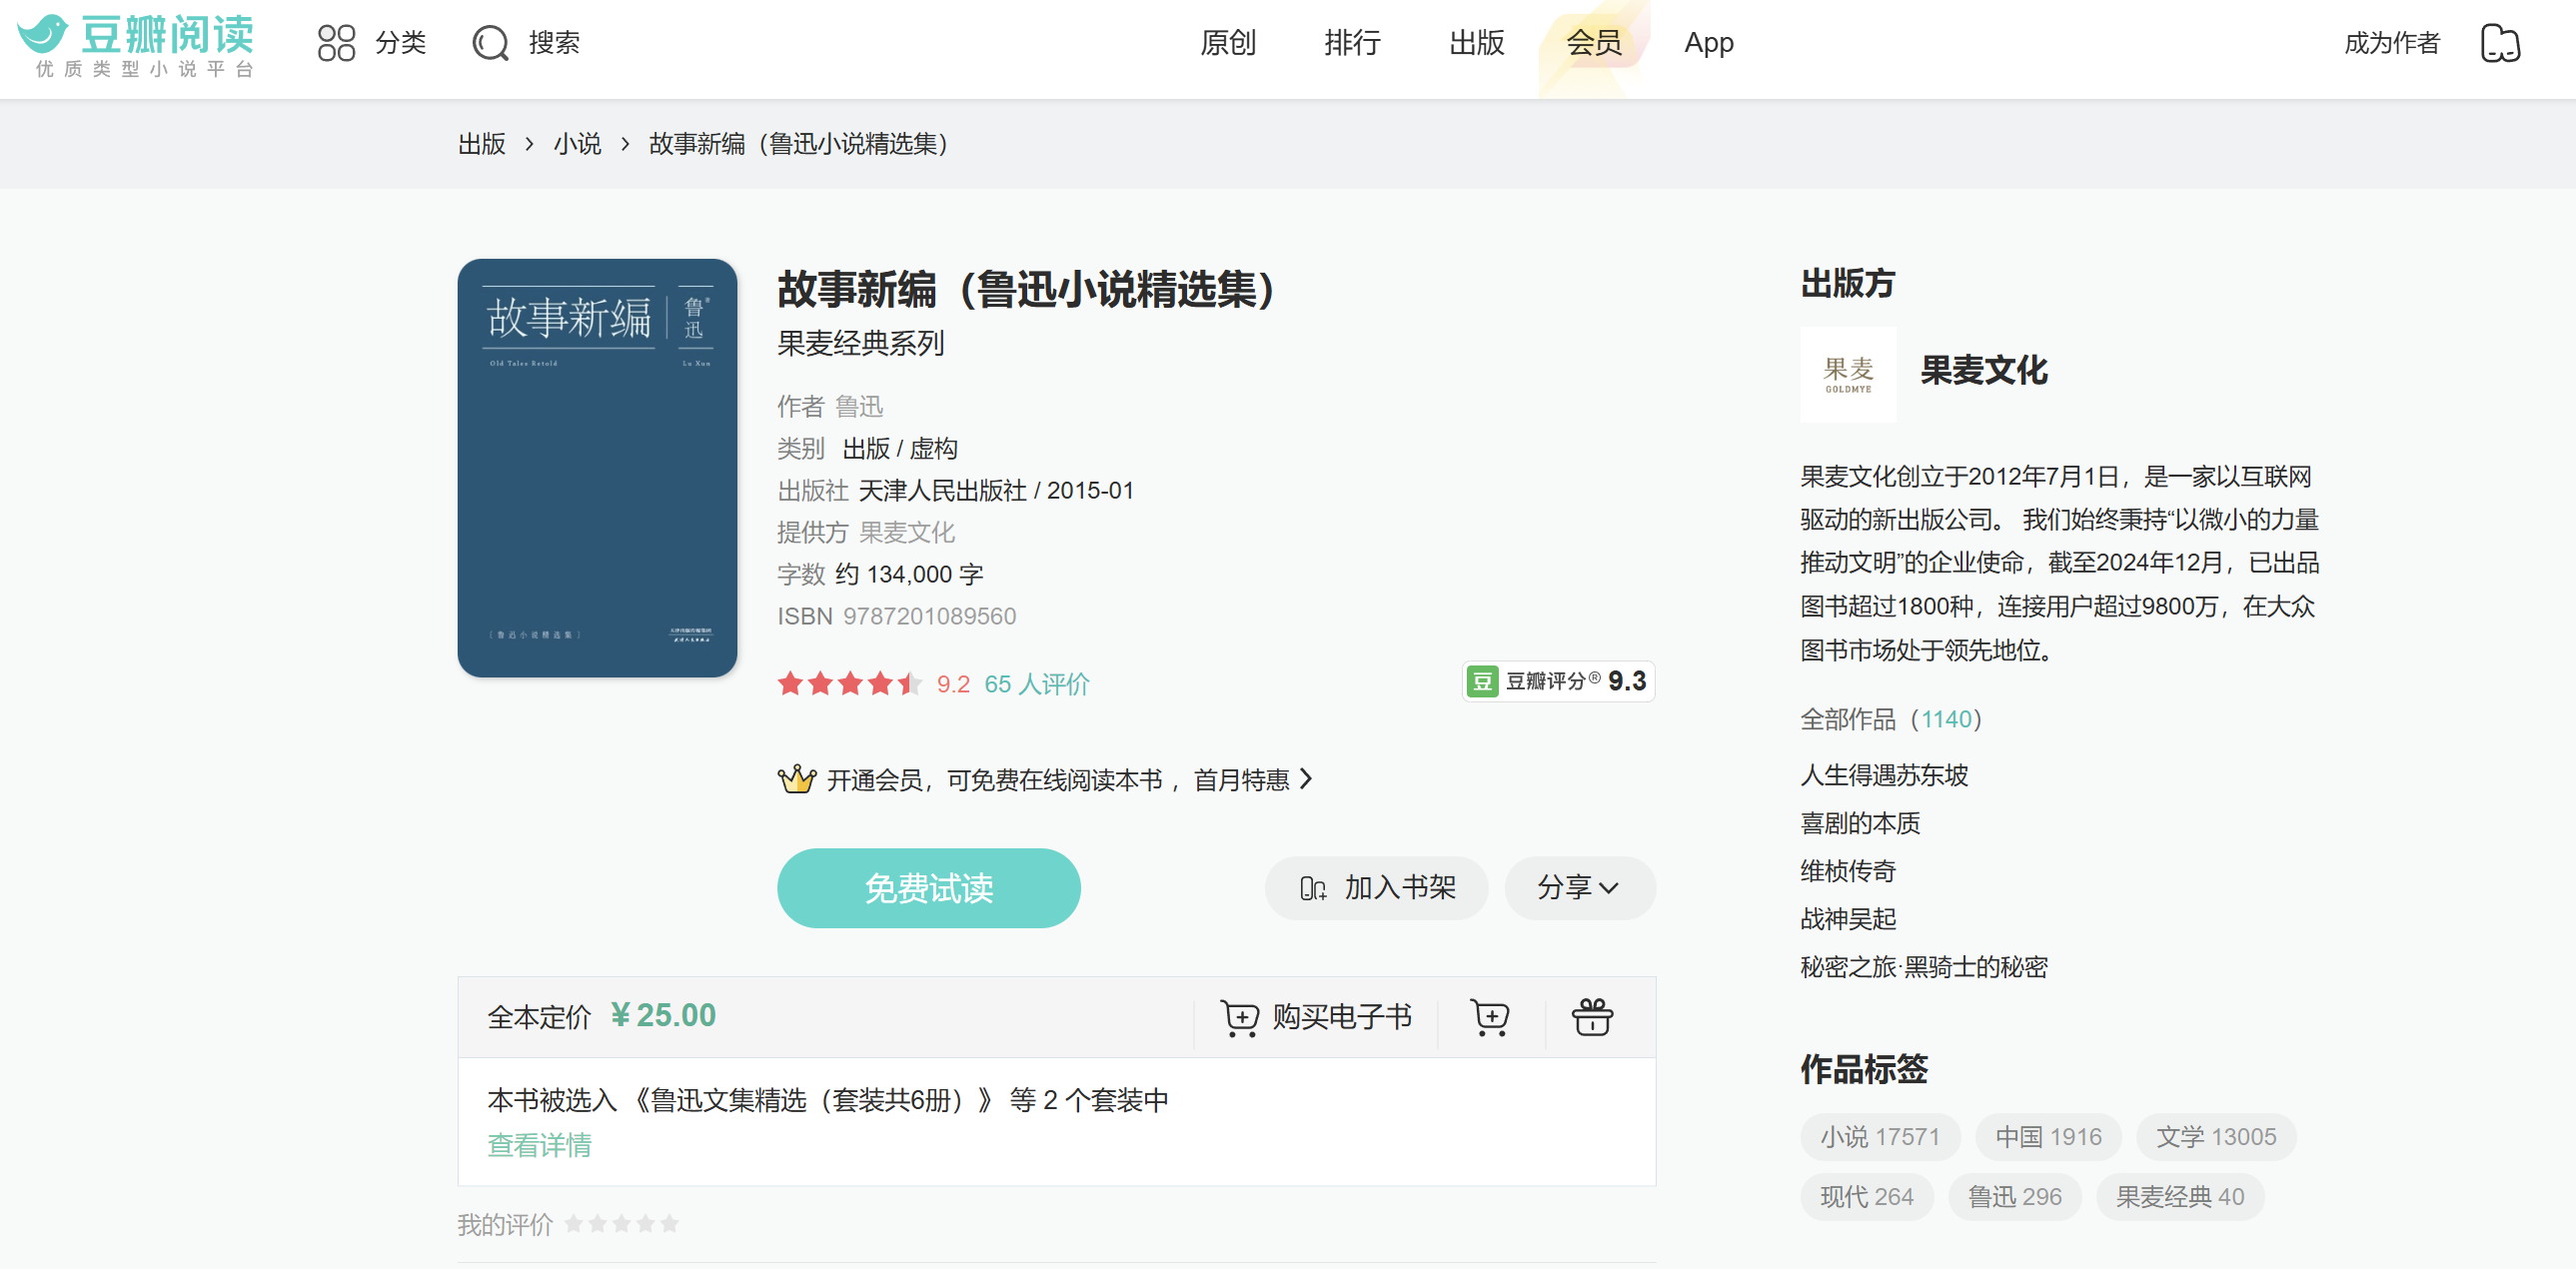
\includegraphics[width=\textwidth]{fig/book3.png} \\
    查看图书详情
  \end{minipage}
  % \hfill
  \begin{minipage}{0.30\textwidth}
    \centering
    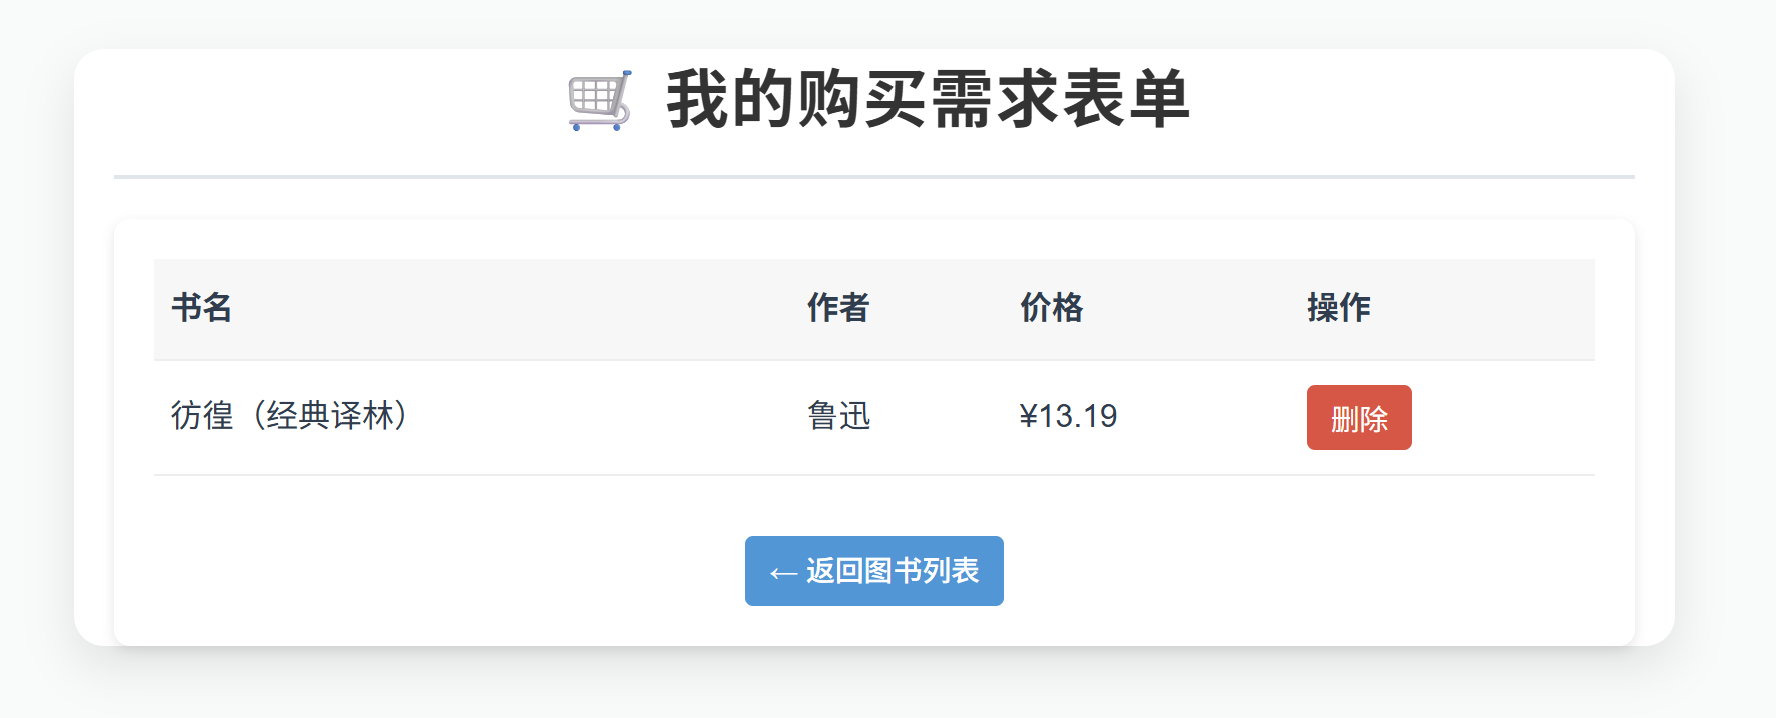
\includegraphics[width=\textwidth]{fig/book4.png} \\
    增删图书
  \end{minipage}
\end{frame}

\section{后端思路}

\subsection{数据库设计}
\begin{frame}{数据库设计}
  
\end{frame}

\subsection{Python-Flask}
\begin{frame}{Python-Flask}
  
\end{frame}

\end{document}
